\subsection{Haptic sensitivity}
\label{Haptic sensitivity}

As the mechanoreceptors are \textbf{enveloped in various skin layers}, their sensitivity to vibrations will not be infinite. The \textbf{strength of the sensation} will depend on the \textbf{frequency} and \textbf{amplitude of the vibration}. 

The \textbf{amplitude} of the vibration can be considered in \textbf{terms of the acceleration of the membrane-magnet system}.

Previous works \cite{Vibrotactile_Sensitivity} found that, for a \textbf{pulp contact area} ranging from \textbf{53 to 176.7 mm\textsuperscript{2}}, the threshold of detection of vibrations was between \textbf{0.1778 and 0.5623 m/s\textsuperscript{2}} (in the work specified as 105-115 dB (re 1e-6m/s\textsuperscript{2})) for sinusoidal stimuli ranging from \textbf{100 to 250 Hz}. 
For frequencies close to \textbf{125Hz} the threshold should also \textbf{lower} as the finger pulp reaches its \textbf{resonance frequency} \cite{Skin_freqs_penetration}.

The study also highlights that the sensitivity depends on the \textbf{constant pressure force applied on the skin} in conjunction with the vibration.
They found that under active pressing force, the sensitivity threshold decreases to 0.027-0.143 m/s\textsuperscript{2} (in the work specified as 68.5-83.1 dB (re 1e-6m/s\textsuperscript{2})) for a constant applied force of 1.6N.

\begin{samepage}
    For higher pressure forces the sensitivity threshold decreases even further, as we can observe in Fig. \ref{fig: Vibrotactile_Sensitivity}.
    \begin{figure}[H]
        \centering
        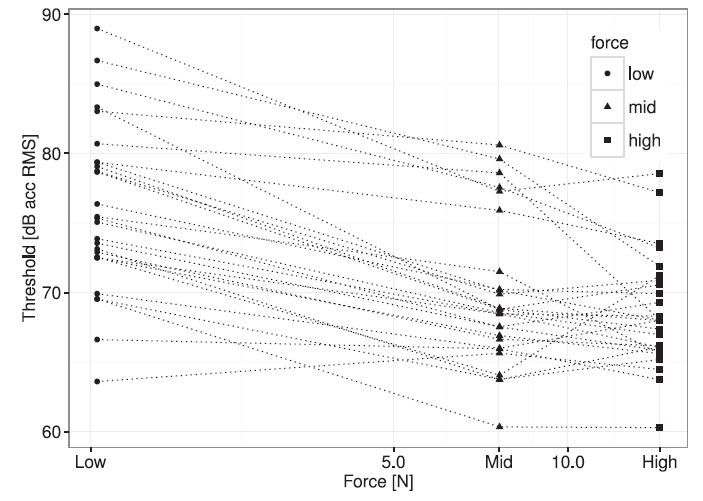
\includegraphics[width=0.5\linewidth]{Chapters/Chapter3/Haptics_Physics/Figures/vibr_thr_vs_pressure_force.png}
        \caption{Sensitivity as a function of the applied pressure \cite{Skin_freqs_penetration}.}
        \label{fig: Vibrotactile_Sensitivity}
    \end{figure}
\end{samepage}

